\subsubsubsubsection{Crossroads}
\begin{figure}[h]
\centering
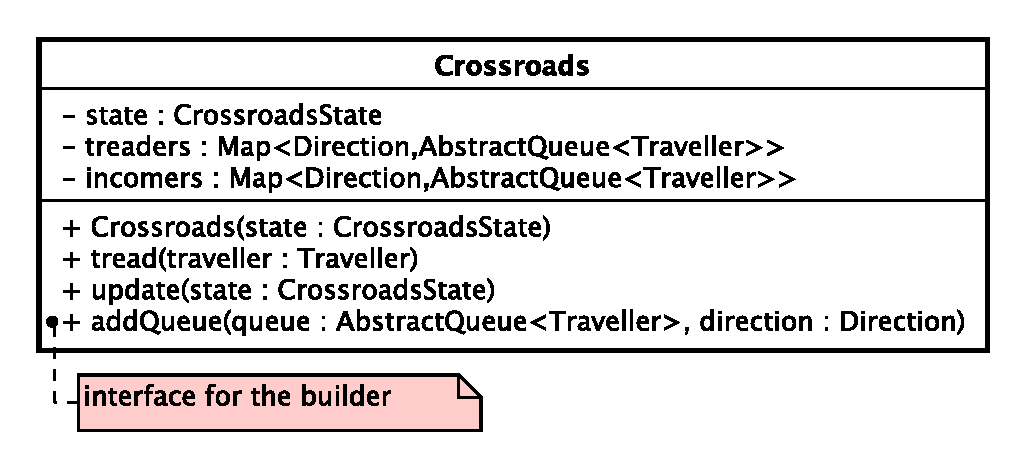
\includegraphics[scale=0.6,keepaspectratio]{images/solution/app/backend/crossroads.eps}
\caption{\pReactiveComponent::Crossroads}
\label{fig:sd-app-crossroads}
\end{figure}
\FloatBarrier
\begin{itemize}
  \item \textbf{\descr} \\
    Protected object that represents a (concrete) crossroads entity.
  \item \textbf{\attrs}
  \begin{itemize}
    \item \texttt{state: CrossroadsState} \\
The traffic light state tells which crossroads' queues can be processed in
order to make waiting vehicles tread the crossroads.
    \item \texttt{treadingAgents: Map<Direction, AbstractQueue<MoveableAgent>>} \\
The queue of urban actors which are treading the crossroads.
    \item \texttt{waitingAgents: Map<Direction, AbstratQueue<MoveableAgent>>} \\
The queue of urban actors which are waiting to tread the crossroads. 
  \end{itemize}
  \item \textbf{\ops}
  \begin{itemize}
    \item[+] \texttt{Crossroads(state : CrossroadsState)} \\
Creates a crossroads specifying its state.
    \item[+] \texttt{tread(agent: MoveableAgent)} \\
Implements the treading of the crossroads.
    \item[+] \texttt{update(state: CrossroadsState)} \\
Updates the state value of the crossroads.
    \item[+] \texttt{addQueue(queue: AbstratQueue<MoveableAgent>, direction: 
Direction)} \\
Add a new queue to waiting and treading maps with the specified direction.
  \end{itemize}
\end{itemize}
